% =====================================================================
% Semana 2 · S2.3 — Puente de Wheatstone (cuarto de puente)
% Fundamentos de Sistemas Electrónicos Analógicos (Ingeniería Aeroespacial)
% Compilar: pdflatex semana_2_s23_puente_wheatstone.tex  (2 pasadas)
% =====================================================================
\documentclass[aspectratio=169]{beamer}

\usepackage[utf8]{inputenc}
\usepackage[T1]{fontenc}
\usepackage{lmodern}
\usepackage[spanish,es-tabla]{babel}
\usepackage{amsmath,amssymb}
\usepackage{siunitx}
\usepackage{booktabs}
\usepackage{microtype}
\usepackage{circuitikz}

\definecolor{navy}{RGB}{23,54,93}
\definecolor{navysoft}{RGB}{72,101,140}
\definecolor{gold}{RGB}{179,142,62}
\definecolor{ink}{RGB}{44,51,58}
\definecolor{soft}{RGB}{244,241,234}

\usetheme{default}
\setbeamertemplate{navigation symbols}{}
\setbeamertemplate{footline}[frame number]
\setbeamercolor{structure}{fg=navy}
\setbeamercolor{frametitle}{fg=white,bg=navy}
\setbeamercolor{title}{fg=navy}
\setbeamercolor{subtitle}{fg=navysoft}
\setbeamercolor{itemize item}{fg=gold}
\setbeamercolor{itemize subitem}{fg=gold}
\setbeamercolor{block title}{fg=white,bg=navy}
\setbeamercolor{block body}{bg=soft}
\setbeamercolor{example text}{fg=navy}
\setbeamertemplate{itemize item}{\scriptsize\raise1.25pt\hbox{\donotcoloroutermaths$\bullet$}}
\setbeamertemplate{itemize subitem}{\scriptsize\raise1.25pt\hbox{\donotcoloroutermaths$\circ$}}
\setbeamerfont{frametitle}{size=\large,series=\bfseries}

\title[S2.3 · Puente de Wheatstone]{Puente de Wheatstone como traductor R–V}
\subtitle{S2.3 — Simulaciones y laboratorio de la Semana 2}
\institute{Licenciatura en Ingeniería Aeroespacial\\ UNAM · ENES Unidad Juriquilla}
\author{M. en C. José de Jesús Santana Ramírez}
\date{Semestre 2027-1}

\begin{document}

% ---------------------------------------------------------------------
\begin{frame}[plain]
  \titlepage
\end{frame}

% ---------------------------------------------------------------------
\begin{frame}{Objetivos de la sesión}
  \begin{itemize}
    \item Construir un \textbf{puente de Wheatstone} como dos divisores y su salida diferencial.
    \item Comprender el \textbf{balanceo} ($V_{diff} = 0$) y el concepto de \emph{cuarto de puente}.
    \item Obtener la \textbf{sensibilidad} $V_{diff} \approx \dfrac{V_{exc}}{4}\cdot\dfrac{dR}{R}$.
    \item Comparar la expresión \textbf{exacta} con la aproximación de pequeña señal.
    \item Evaluar la \textbf{potencia} de la rama sensora (autocalentamiento).
  \end{itemize}
  \pause
  \begin{block}{Pregunta}
    ¿Por qué el puente mide la deformación de un sensor y no su resistencia absoluta?
  \end{block}
\end{frame}

% ---------------------------------------------------------------------
\begin{frame}{Teoría 1 · El puente como dos divisores}
  Un puente se construye con dos divisores de tensión que comparten la excitación $V_{exc}$:
  \[
    V_{diff} = V_{left} - V_{right}
    \qquad
    V_{left} = V_{exc}\cdot\frac{R_2}{R_1+R_2}
    \qquad
    V_{right} = V_{exc}\cdot\frac{R_4}{R_3+R_4}
  \]
  \begin{center}
    \resizebox{0.72\linewidth}{!}{%
    \begin{circuitikz}[american voltages, scale=0.95]
      \draw (0,3) to[V, l={$V_{exc}$}, i=$I$] (0,0);
      \draw (0,3) -- (7.6,3);
      \draw (0,0) -- (7.6,0);
      \draw (1.8,3) to[R, l={$R_1$}] (1.8,1.5);
      \draw (1.8,1.5) to[R, l={$R_2$}] (1.8,0);
      \node[circle, fill=gold, inner sep=0.9pt] at (1.8,1.5) {};
      \node[above, text=gold] at (1.8,1.78) {$V_{left}$};
      \draw (5.8,3) to[R, l={$R_3$}] (5.8,1.5);
      \draw (5.8,1.5) to[R, l={$R_4$}] (5.8,0);
      \node[circle, fill=gold, inner sep=0.9pt] at (5.8,1.5) {};
      \node[above, text=gold] at (5.8,1.78) {$V_{right}$};
    \node[ground] at (0,0) {};
    \end{circuitikz}}
  \end{center}
\end{frame}

% ---------------------------------------------------------------------
\begin{frame}{Teoría 2 · Balance y sensibilidad}
  \begin{itemize}
    \item Con cuatro resistores iguales, el puente está \textbf{balanceado}: $V_{left}=V_{right}$ $\Rightarrow$ $V_{diff} = 0$ V.
    \item Si un solo resistor cambia de $R$ a $R+dR$ (\emph{cuarto de puente}) y $|dR|\ll R$:
  \end{itemize}
  \[
    V_{diff} \approx \frac{V_{exc}}{4}\cdot\frac{dR}{R}
  \]
  \pause
  \begin{itemize}
    \item La \textbf{sensibilidad} es $V_{exc}/4$: un cambio de $1\,\text{\%}$ en la rama da
      $V_{exc}/4 \cdot 0.01$ de salida.
    \item La salida es proporcional a la \emph{deformación} (resistiva), no al valor absoluto;
      el puente rechaza el modo común (temperatura) y detecta la diferencia.
  \end{itemize}
\end{frame}

% ---------------------------------------------------------------------
\begin{frame}{Ejercicio · Enunciado}
  \begin{block}{Cuarto de puente de la simulación S2.3}
    \centering
    $V_{exc} = \SI{5}{\volt}$, \quad $R_1 = R_2 = R_3 = R_4 = 1\,\text{k}\Omega$, \quad $\Delta$ de $-1\,\text{\%}$ a $+1\,\text{\%}$ en $R_1$.
  \end{block}
  \begin{center}
    \resizebox{0.72\linewidth}{!}{%
    \begin{circuitikz}[american voltages, scale=0.95]
      \draw (0,3) to[V, l={$V_{exc}=5\,\mathrm{V}$}, i=$I$] (0,0);
      \draw (0,3) -- (7.6,3);
      \draw (0,0) -- (7.6,0);
      \draw (1.8,3) to[R, l={$R_1$}] (1.8,1.5);
      \draw (1.8,1.5) to[R, l={$R_2$}] (1.8,0);
      \node[circle, fill=gold, inner sep=0.9pt] at (1.8,1.5) {};
      \node[above, text=gold] at (1.8,1.7) {$V_{left}$};
      \draw (5.8,3) to[R, l={$R_3$}] (5.8,1.5);
      \draw (5.8,1.5) to[R, l={$R_4$}] (5.8,0);
      \node[circle, fill=gold, inner sep=0.9pt] at (5.8,1.5) {};
      \node[above, text=gold] at (5.8,1.78) {$V_{right}$};
    \node[ground] at (0,0) {};
    \end{circuitikz}}
  \end{center}
  \textbf{Determinar:} $V_{diff}$ en balance y para $\Delta = +1\,\text{\%}$ y $\Delta = -1\,\text{\%}$; la pendiente y la potencia de la rama.
\end{frame}

% ---------------------------------------------------------------------
\begin{frame}{Desarrollo · Paso 1 — Balance}
  Con $R_1=R_2=R_3=R_4$ y $\Delta = 0$:
  \[
    V_{left} = V_{right} = 5\cdot\frac{1000}{1000+1000} = \SI{2.500}{\volt}
    \qquad\Longrightarrow\qquad
    \boxed{\;V_{diff} = 0\ \text{V}\;}
  \]
  \pause
  \begin{itemize}
    \item El puente balanceado da salida nula: no hay que restar una gran componente común.
    \item Esta es la ventaja frente a un divisor único: la referencia es la otra mitad del puente.
  \end{itemize}
\end{frame}

% ---------------------------------------------------------------------
\begin{frame}{Desarrollo · Paso 2 — $\Delta = +1\,\text{\%}$}
  \begin{align*}
    V_{left} &= 5\cdot\frac{1\,\text{k}}{1\,\text{k}(1.01)+1\,\text{k}} = \SI{2.4876}{\volt}\\
    V_{right} &= \SI{2.500}{\volt}\\
    V_{diff} &= 2.4876 - 2.500 = -\SI{12.44}{\milli\volt}
  \end{align*}
  \pause
  \begin{itemize}
    \item $R_1$ sube $\Rightarrow$ $V_{left}$ baja $\Rightarrow$ $V_{diff}$ negativo (según la convención $V_{left}-V_{right}$).
    \item \textbf{El signo importa}: indica la dirección de la deformación (tensión o compresión).
  \end{itemize}
\end{frame}

% ---------------------------------------------------------------------
\begin{frame}{Desarrollo · Paso 3 — $\Delta = -1\,\text{\%}$}
  \begin{align*}
    V_{left} &= 5\cdot\frac{1\,\text{k}}{1\,\text{k}(0.99)+1\,\text{k}} = \SI{2.5126}{\volt}\\
    V_{right} &= \SI{2.500}{\volt}\\
    V_{diff} &= 2.5126 - 2.500 = +\SI{12.56}{\milli\volt}
  \end{align*}
  \pause
  \begin{itemize}
    \item $R_1$ baja $\Rightarrow$ $V_{left}$ sube $\Rightarrow$ $V_{diff}$ positivo.
    \item Amplitud simétrica ($\approx \pm 12.5\,\text{mV}$ para $\pm 1\,\text{\%}$): el puente es casi lineal en pequeña señal.
  \end{itemize}
\end{frame}

% ---------------------------------------------------------------------
\begin{frame}{Desarrollo · Paso 4 — Sensibilidad: exacto contra aproximación}
  \begin{align*}
    \text{exacto: } V_{diff}(+1\,\text{\%}) &= -\SI{12.44}{\milli\volt}\\[2pt]
    \text{aprox: } V_{diff} &\approx \frac{V_{exc}}{4}\cdot\Delta = \frac{5}{4}\cdot 0.01 = \SI{12.5}{\milli\volt}
  \end{align*}
  \pause
  \begin{block}{Conclusión de modelo}
    La pendiente cerca del balance es $\approx V_{exc}/4 = \SI{1.25}{\volt}$ \textbf{por unidad} de $\Delta$
    (o $\SI{12.5}{\milli\volt}$ por $1\,\text{\%}$). La aproximación lineal es válida para $|dR/R| \lesssim 1\,\text{\%}$.
    La expresión exacta difiere de la lineal en el término de segundo orden.
  \end{block}
\end{frame}

% ---------------------------------------------------------------------
\begin{frame}{Desarrollo · Paso 5 — Potencia de la rama sensora}
  La rama $R_1$ disipa:
  \[
    P_{R1} = \frac{\left(V_{exc} - V_{left}\right)^2}{R_1(1+\Delta)}
    \approx \frac{(5-2.5)^2}{1000} = \SI{6.25}{\milli\watt}
  \]
  \pause
  \begin{itemize}
    \item En el equilibrio, cada rama disipa $\approx \SI{6.25}{\milli\watt}$ (con $1\,\text{k}\Omega$ y $5\,\text{V}$).
    \item Si la excitación sube, la señal crece $\propto V_{exc}$ pero la potencia $\propto V_{exc}^2$: compromiso señal/autocalentamiento.
    \item Con una \emph{galga} de $350\,\Omega$ y $5\,\text{V}$, la potencia por rama es mayor
      ($\approx 17.9\,\text{mW}$), y el autocalentamiento debe presupuestarse.
  \end{itemize}
\end{frame}

% ---------------------------------------------------------------------
\begin{frame}[fragile]{Verificación en LTspice}
  Abrir \texttt{semana2\_03\_wheatstone\_desbalance.cir} (barrido de $\Delta$ de $-0.01$ a $0.01$ en pasos de $0.001$)
  y consultar el Error Log:

  \begin{verbatim}
.meas op VLEFT  FIND V(left)
.meas op VRIGHT FIND V(right)
.meas op VDIFF  PARAM V(left)-V(right)
.meas op P_R1   PARAM (V(top)-V(left))*(V(top)-V(left))/(1000*(1+DELTA))
  \end{verbatim}

  \textbf{Criterio de éxito:} $V_{diff} \approx 0$ en balance; $\approx \mp 12.5\,\text{mV}$ para
  $\Delta = \pm 1\,\text{\%}$; pendiente $\approx V_{exc}/4$.
\end{frame}

% ---------------------------------------------------------------------
  % ---------------------------------------------------------------------
  \begin{frame}{Resultado de la simulación}
    \begin{center}
      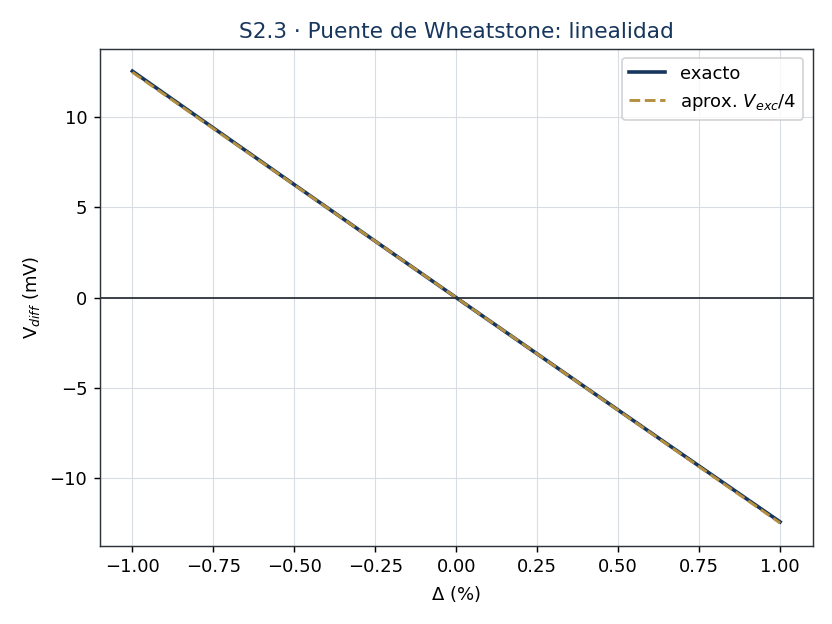
\includegraphics[width=0.78\textwidth]{figs/s23_puente.png}
    \end{center}
    \begin{itemize}
      \item La salida es casi lineal cerca del balance (pendiente $V_{exc}/4$) y el signo indica la dirección.
    \end{itemize}
  \end{frame}

  % ---------------------------------------------------------------------
  \begin{frame}{Errores comunes}
  \begin{table}
    \small
    \begin{tabular}{p{0.34\textwidth}p{0.30\textwidth}p{0.30\textwidth}}
      \toprule
      Error & Consecuencia & Corrección \\
      \midrule
      Usar la salida de una sola rama & Incluir el modo común & Medir $V_{diff}$ (diferencial) \\
      Ignorar el signo de $V_{diff}$ & No saber la dirección de deformación & Fijar la convención $V_{left}-V_{right}$ \\
      Aplicar la aprox lineal a $\Delta$ grande & Error de no linealidad & $|dR/R| \lesssim 1\,\text{\%}$ \\
      No presupuestar el autocalentamiento & Deriva térmica del sensor & Limitar $V_{exc}$ según potencia \\
      Mezclar cuarto, medio y puente completo & Sensibilidad distinta & Usar $V_{exc}/4$ (cuarto), $V_{exc}/2$ (medio) \\
      \bottomrule
    \end{tabular}
  \end{table}
\end{frame}

% ---------------------------------------------------------------------
\begin{frame}{Lectura aeroespacial}
  \begin{itemize}
    \item \textbf{Galga extensométrica:} el puente convierte la deformación estructural en tensión
      diferencial; la señal típica es de milivolts y requiere amplificación de precisión.
    \item \textbf{Rechazo de modo común:} la temperatura afecta a las cuatro ramas por igual
      (\emph{common-mode}); la salida diferencial la rechaza, pero el desbalance entre ramas (\emph{tracking}) no.
    \item \textbf{Autocalentamiento y vacío:} sin convección, la potencia disipada en la rama calienta
      la galga; se limita la excitación y se documenta la deriva.
    \item \textbf{Ficha de interfaz:} antes de amplificar se documentan rango de $V_{diff}$ (con signo),
      tensión de modo común, $R_{out}$ de cada rama, tolerancia y deriva, y la impedancia de entrada requerida.
  \end{itemize}
\end{frame}

% ---------------------------------------------------------------------
\begin{frame}{Preguntas de verificación}
  \begin{enumerate}
    \item ¿Por qué la salida del puente es diferencial y ventaja frente a un divisor único?
    \item ¿Qué pendiente tiene $V_{diff}$ respecto de $\Delta$ cerca del balance?
      \uncover<2->{\emph{$(\approx V_{exc}/4 = \SI{1.25}{\volt}$ por unidad.)}}
    \item Si $\Delta = +1\,\text{\%}$, ¿$V_{diff}$ es positivo o negativo?
      \uncover<3->{\emph{(Negativo con la convención $V_{left}-V_{right}$.)}}
    \item ¿Por qué el autocalentamiento limita la excitación?
      \uncover<4->{\emph{($P \propto V_{exc}^2$; la señal solo $\propto V_{exc}$.)}}
    \item ¿Qué diferencia hay entre cuarto, medio y puente completo en sensibilidad?
  \end{enumerate}
\end{frame}


\end{document}
